\chapter[Amplitude Modulation- Generation]{Amplitude Modulation- Generation}

\section*{Aim}
To design and set-up  an AM generator using BJT and measure the modulation index from the observed output waveform.

\section*{Theory}
\paragraph{}
	The transistor $T_1$ is configured as a common emitter amplifier. The RF carrier wave is given at the base through a coupling capacitor $C_1$.  The message signal used for modulation is the AF signal applied between the emitter resistance and the ground. The message signal modulates the envelope of the carrier which is obtained as output from the collector through a coupling capacitor $C_3$. 
\paragraph{}
The ratio of the maximum amplitude of the modulating signal voltage to that of the carrier voltage is termed as modulation index. This is represented as $m=\frac{V_m}{V_c}$.


\section*{Design}
\textcolor{red}{Design steps need to be verified}

\paragraph{DC Biasing conditions:}
Choose BF194 which is a high frequency transistor. From its datasheet (See \ref{BF194/195}) the various parameters can be obtained as:

 
Let the supply voltage be 60\% of the maximum $V_{ce}$.  \begin{equation}
V_{cc}=\ 60\% of V_{cemax}=\ 12 V
\end{equation}

\noindent Let the collector current $I_c$ be 10\% of maximum rated value.
\begin{equation}
I_{c}=\ 3\% \ of \ I_{cmax}=\ 1 mA
\end{equation}

\noindent In-order to fix the biasing point in the middle of load line, let $V_{RC}$ be 40\% of $V_{cc}$, $V_{RE}$\ be\ 10\% \ of $V_{cc}$ and $V_{ce}$\  be\ 50\% \ of $V_{cc}$.
\begin{equation}
V_{RC}=\ 45\% \ of \ V_{cc}=\ 5.4V
\end{equation}
\begin{equation}
V_{RE}=\ 5\% \ of \ V_{cc}=\ 0.6V
\end{equation}
\begin{equation}
V_{ce}=\ 50\% \ of \ V_{cc}=\ 6V
\end{equation}
\paragraph{Design of Resistors:}
\begin{equation}
R_C=\frac{V_{RC}}{I_c}=\ \frac{5.4V}{1mA}=\ 5.4 k\Omega
\end{equation}
\begin{equation}
R_E=\frac{V_{RE}}{I_e}=\ \frac{0.6V}{1mA}=\ 600\Omega
\end{equation}
\noindent From the datasheet, hFE has a minium value of 67. 
\begin{equation}
I_b=\frac{I_c}{hFE}=\frac{1mA}{67}=\ 15 \mu A
\end{equation}
\noindent Assume the current through $R_1=\ 10 I_b$ and that through $R_2=9I_b$ 
\begin{equation}
 V_{R2}=V_{be}+V_{RE}\\ =0.7+0.6V=1.3V
\end{equation}
\noindent Then
\begin{equation}
R_2=\frac{V_{R2}}{9I_b}=\frac{1.2V}{9X15X10^{-6}}=8.8 k\Omega
\end{equation}
\noindent and 
\begin{equation}
R_1=\frac{V_{R1}}{10I_b}=\frac{10.8V}{10X15X10{^-6}}= 72k\Omega
\end{equation}

\noindent Based on these design equations use the standard resistor values of $R_1=22k\Omega,\ R_2=10k\Omega, \ R_c=10k\Omega,\ R_c=560\Omega$ and a load resistance of $R_L=1k\Omega$.
Use coupling capacitors $C_1=0.1 \mu F,\ C_2=0.001\mu F$ and emitter bye-pass capacitor $C_E=0.01\mu F$.
\section*{Components and Equipments Required}
Function Generators(2), CRO(2), Connection wires, Breadboard, Probes.
\\BF194 - High frequency bipolar junction transistor
\\ $22k\Omega,\  10k\Omega\ (2),\ 560\Omega,\,\ 1k\Omega $ - Resistors
\\ $ 0.1\mu F,\ 0.01\mu F, \ 0.001\mu F $ - Capacitors
\\ 
\section*{Circuit Diagram}
\begin{figure}[h]
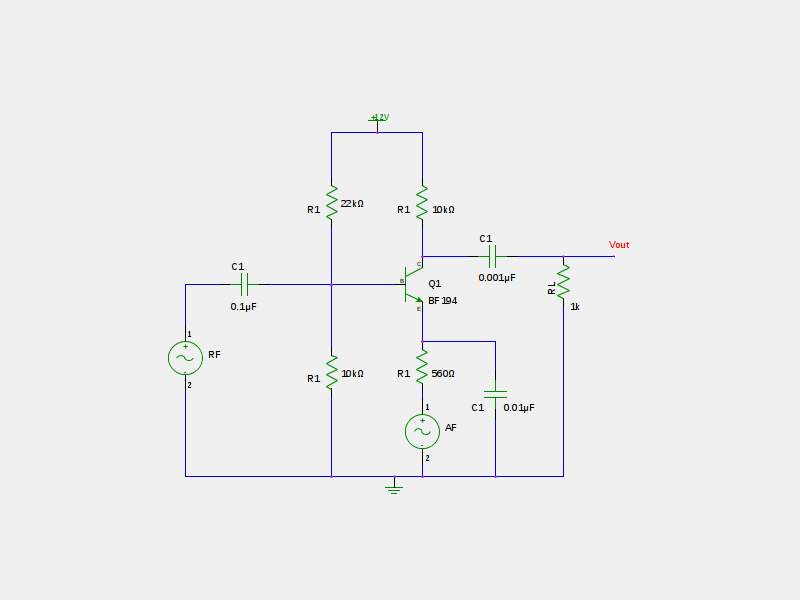
\includegraphics[width=15cm, height=10cm, trim=5cm 3.5cm 4cm 3.5cm, clip=true]{AM.png}
\caption{Circuit Diagram for Amplitude modulation using BJT}

\end{figure}

\section*{Procedure}
\begin{enumerate}
\item
Set up the circuit after verifying the condition of components.
\item
Feed AF modulating signal (say, $f_m=1kHz$ and $E_m=150mV$) and Rf carrier (say, $f_c=70kHz$ and $E_c=300mV$) using function generators.
\item
Adjust amplitude and frequencies of the AF and RF signals and observe amplitude modulated waveform on the CRO.
\item
Fix $f_m$ and $f_c$. Note down $E_{max}$ and $E_{min}$ of the AM signal and calculate modulation index according to the formula ,
\begin{equation}
m=\frac{E_{max}-E_{min}}{E_{max}+E_{min}}.
\end{equation}
Here $E_{max}$ is the maximum of the positive envelope of the carrier and $E_{min}$ is the minimum of the positivee envelope of the carrier.
\item
Repeat for different values of $E_m$ and $E_c$. Observe the AM waveforms for different values of m.
\item
Plot the waveforms on a graph sheet.
\item

Fill in the observation column
\end{enumerate}


\section*{Observation}


\begin{figure}[h]

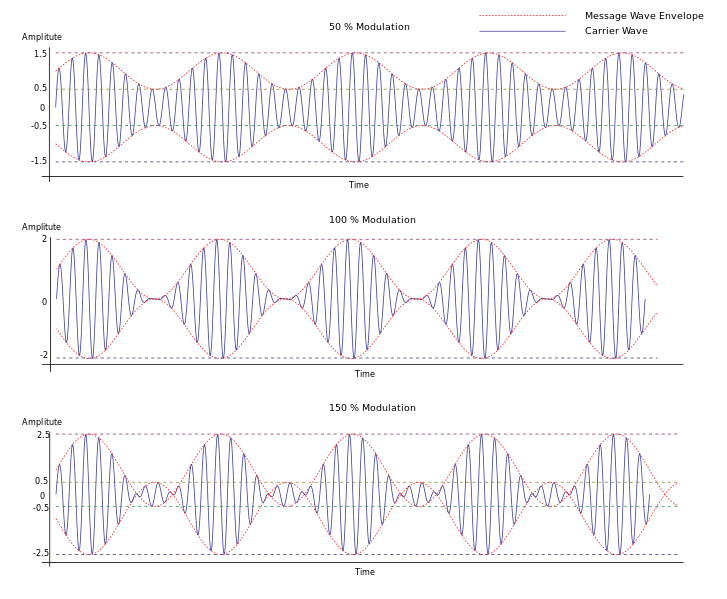
\includegraphics[width=\textwidth]{AMmodindex.png}
\caption{Effect of modulation index on AM}
\label{AMmodindex}
\end{figure}
\noindent Fig \ref{AMmodindex}  shows the effect of modulation index on the resultant AM wave\footnote{\url{https://commons.wikimedia.org:/wiki/File:Amplitude_Modulated_Wave-hm-64.svg}}
\begin{center}

\begin{tabular}{|l|l|l|}

\hline
 & &\\
 
$E_{min}$  & $E_{max}$ & $m=\frac{E_{max}-E_{min}}{E_{max}+E_{min}}$ \\
 & & \\ \hline
 & & \\ \hline
& & \\ \hline
& & \\ \hline
& & \\ \hline
& & \\ \hline

\end{tabular}
\end{center}


\section*{Result}

Implemented the AM modulation circuit using BJT.
The modulation index corresponding to $E_m=$ \textemdash \textemdash and $E_c=$ \textemdash\textemdash is : m= \textemdash\textemdash .
